%%
%% This is file `sample-acmtog.tex',
%% generated with the docstrip utility.
%%
%% The original source files were:
%%
%% samples.dtx  (with options: `all,journal,bibtex,acmtog')
%% 
%% IMPORTANT NOTICE:
%% 
%% For the copyright see the source file.
%% 
%% Any modified versions of this file must be renamed
%% with new filenames distinct from sample-acmtog.tex.
%% 
%% For distribution of the original source see the terms
%% for copying and modification in the file samples.dtx.
%% 
%% This generated file may be distributed as long as the
%% original source files, as listed above, are part of the
%% same distribution. (The sources need not necessarily be
%% in the same archive or directory.)
%%
%%
%% Commands for TeXCount
%TC:macro \cite [option:text,text]
%TC:macro \citep [option:text,text]
%TC:macro \citet [option:text,text]
%TC:envir table 0 1
%TC:envir table* 0 1
%TC:envir tabular [ignore] word
%TC:envir displaymath 0 word
%TC:envir math 0 word
%TC:envir comment 0 0
%%
%%
%% The first command in your LaTeX source must be the \documentclass
%% command.
%%
%% For submission and review of your manuscript please change the
%% command to \documentclass[manuscript, screen, review]{acmart}.
%%
%% When submitting camera ready or to TAPS, please change the command
%% to \documentclass[sigconf]{acmart} or whichever template is required
%% for your publication.
%%
%%
\documentclass[acmtog]{acmart}

%%
%% \BibTeX command to typeset BibTeX logo in the docs
\AtBeginDocument{%
  \providecommand\BibTeX{{%
    Bib\TeX}}}

%% Rights management information.  This information is sent to you
%% when you complete the rights form.  These commands have SAMPLE
%% values in them; it is your responsibility as an author to replace
%% the commands and values with those provided to you when you
%% complete the rights form.
\setcopyright{acmlicensed}
\copyrightyear{2018}
\acmYear{2018}
\acmDOI{XXXXXXX.XXXXXXX}


%%
%% These commands are for a JOURNAL article.
\acmJournal{TOG}
\acmVolume{37}
\acmNumber{4}
\acmArticle{111}
\acmMonth{8}

%%
%% Submission ID.
%% Use this when submitting an article to a sponsored event. You'll
%% receive a unique submission ID from the organizers
%% of the event, and this ID should be used as the parameter to this command.
%%\acmSubmissionID{123-A56-BU3}

%%
%% For managing citations, it is recommended to use bibliography
%% files in BibTeX format.
%%
%% You can then either use BibTeX with the ACM-Reference-Format style,
%% or BibLaTeX with the acmnumeric or acmauthoryear sytles, that include
%% support for advanced citation of software artefact from the
%% biblatex-software package, also separately available on CTAN.
%%
%% Look at the sample-*-biblatex.tex files for templates showcasing
%% the biblatex styles.
%%

%%
%% The majority of ACM publications use numbered citations and
%% references.  The command \citestyle{authoryear} switches to the
%% "author year" style.
%%
%% If you are preparing content for an event
%% sponsored by ACM SIGGRAPH, you must use the "author year" style of
%% citations and references.
\citestyle{acmauthoryear}


%%
%% end of the preamble, start of the body of the document source.
\begin{document}

%%
%% The "title" command has an optional parameter,
%% allowing the author to define a "short title" to be used in page headers.
\title{The Name of the Title Is Hope}

%%
%% The "author" command and its associated commands are used to define
%% the authors and their affiliations.
%% Of note is the shared affiliation of the first two authors, and the
%% "authornote" and "authornotemark" commands
%% used to denote shared contribution to the research.
\author{Ben Trovato}
\authornote{Both authors contributed equally to this research.}
\email{trovato@corporation.com}
\orcid{1234-5678-9012}
\author{G.K.M. Tobin}
\authornotemark[1]
\email{webmaster@marysville-ohio.com}
\affiliation{%
  \institution{Institute for Clarity in Documentation}
  \city{Dublin}
  \state{Ohio}
  \country{USA}
}

\author{Lars Th{\o}rv{\"a}ld}
\affiliation{%
  \institution{The Th{\o}rv{\"a}ld Group}
  \city{Hekla}
  \country{Iceland}}
\email{larst@affiliation.org}

\author{Valerie B\'eranger}
\affiliation{%
  \institution{Inria Paris-Rocquencourt}
  \city{Rocquencourt}
  \country{France}
}

\author{Aparna Patel}
\affiliation{%
 \institution{Rajiv Gandhi University}
 \city{Doimukh}
 \state{Arunachal Pradesh}
 \country{India}}

\author{Huifen Chan}
\affiliation{%
  \institution{Tsinghua University}
  \city{Haidian Qu}
  \state{Beijing Shi}
  \country{China}}

\author{Charles Palmer}
\affiliation{%
  \institution{Palmer Research Laboratories}
  \city{San Antonio}
  \state{Texas}
  \country{USA}}
\email{cpalmer@prl.com}

\author{John Smith}
\affiliation{%
  \institution{The Th{\o}rv{\"a}ld Group}
  \city{Hekla}
  \country{Iceland}}
\email{jsmith@affiliation.org}

\author{Julius P. Kumquat}
\affiliation{%
  \institution{The Kumquat Consortium}
  \city{New York}
  \country{USA}}
\email{jpkumquat@consortium.net}

%%
%% By default, the full list of authors will be used in the page
%% headers. Often, this list is too long, and will overlap
%% other information printed in the page headers. This command allows
%% the author to define a more concise list
%% of authors' names for this purpose.
\renewcommand{\shortauthors}{Trovato et al.}

%%
%% The abstract is a short summary of the work to be presented in the
%% article.
\begin{abstract}
  A clear and well-documented \LaTeX\ document is presented as an
  article formatted for publication by ACM in a conference proceedings
  or journal publication. Based on the ``acmart'' document class, this
  article presents and explains many of the common variations, as well
  as many of the formatting elements an author may use in the
  preparation of the documentation of their work.
\end{abstract}

%%
%% The code below is generated by the tool at http://dl.acm.org/ccs.cfm.
%% Please copy and paste the code instead of the example below.
%%
\begin{CCSXML}
<ccs2012>
 <concept>
  <concept_id>00000000.0000000.0000000</concept_id>
  <concept_desc>Do Not Use This Code, Generate the Correct Terms for Your Paper</concept_desc>
  <concept_significance>500</concept_significance>
 </concept>
 <concept>
  <concept_id>00000000.00000000.00000000</concept_id>
  <concept_desc>Do Not Use This Code, Generate the Correct Terms for Your Paper</concept_desc>
  <concept_significance>300</concept_significance>
 </concept>
 <concept>
  <concept_id>00000000.00000000.00000000</concept_id>
  <concept_desc>Do Not Use This Code, Generate the Correct Terms for Your Paper</concept_desc>
  <concept_significance>100</concept_significance>
 </concept>
 <concept>
  <concept_id>00000000.00000000.00000000</concept_id>
  <concept_desc>Do Not Use This Code, Generate the Correct Terms for Your Paper</concept_desc>
  <concept_significance>100</concept_significance>
 </concept>
</ccs2012>
\end{CCSXML}

\ccsdesc[500]{Do Not Use This Code~Generate the Correct Terms for Your Paper}
\ccsdesc[300]{Do Not Use This Code~Generate the Correct Terms for Your Paper}
\ccsdesc{Do Not Use This Code~Generate the Correct Terms for Your Paper}
\ccsdesc[100]{Do Not Use This Code~Generate the Correct Terms for Your Paper}

%%
%% Keywords. The author(s) should pick words that accurately describe
%% the work being presented. Separate the keywords with commas.
\keywords{Do, Not, Us, This, Code, Put, the, Correct, Terms, for,
  Your, Paper}

\received{20 February 2007}
\received[revised]{12 March 2009}
\received[accepted]{5 June 2009}

%%
%% This command processes the author and affiliation and title
%% information and builds the first part of the formatted document.
\maketitle

\section{Introduzione}
\input{capitoli/introduzione.tex}

\section{Identificazione dei giocatori e team classification}
\input{capitoli/player.tex}

\section{Prospettiva e Omografia}
\documentclass{article}
\usepackage{graphicx} % Required for inserting images
\usepackage{subcaption}


\author{Simone La Bella}
\date{May 2024}

\begin{document}


\section{Omografia e calcolo prospettiva}
Una parte fondamentale del progetto è stata la calibrazione della camera, in particolare era importante capire o simulare il grandangolo e il fuoco della lente. L'obiettivo finale era quello di mappare le posizioni all'interno dell'immagine data in input, con la posizione relativa in un campo da calcio 2D, tramite una \textbf{matrice di omografia} [link wikipedia]. 
Questo passaggio è fondamentale ai fini della riuscita del progetto, per rendere più veloce il calcolo del fuorigioco e per dare piu informazioni all'utente. Sono state percorse varie idee, prima di arrivare alla soluzione finale.
\\
\subsection{Approci sperimentali}
La prima è stata quella di effettuare una maschera sul campo tramite OpenCV, in modo da eliminare gli spalti per avere meno informazioni superflue possibili, che avrebbero potuto alterare il risultato. [Fig 1]  

\begin{figure}[h]
    \centering
    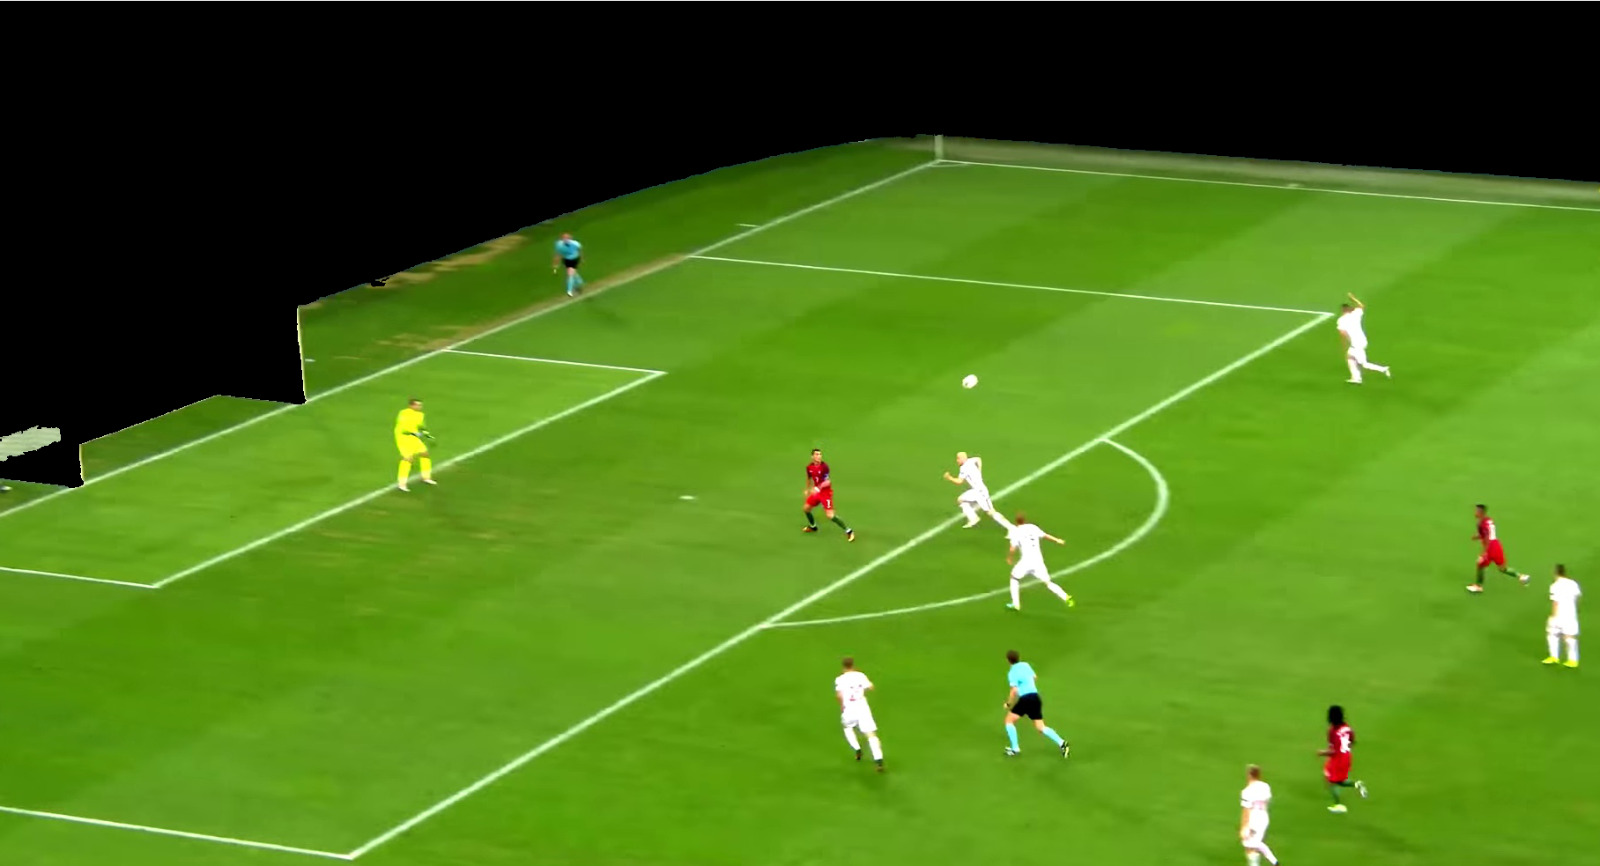
\includegraphics[width=0.7\linewidth]{capitoli/senzaSpalti.jpg}
    \caption{Immagine risultante dopo l'eliminazione degl spalti tramite maschere e operazioni bitwise}
    \label{fig:enter-label}
\end{figure}

In seguito alla maschera sono state effettuate delle operazioni sull'immagine in modo da pre-processarla [Fig 2a], per migliorare la possibilità di individuare le linee del campo tramite la funzione \textbf{RoughLinesP()} [link documentazione OpenCV], per individuare 4 punti, non su una stessa linea, che ci avrebbero permesso di calcolare la matrice di omografia dell'immagine, in modo da poter mappare i punti su un immagine 2D. Il problema di questo metodo si riscontra nella radice del nostro progetto, ovvero le immagini del campo, che essendo di una qualità non elevata, rendevano impossibile per la funzione individuare in maniera netta le linee, anche se ad occhio umano sarebbero potute sembrare ben delineate. [Fig 2b] 

\begin{figure}[h]
    \centering
    \begin{subfigure}{0.33\textwidth}
        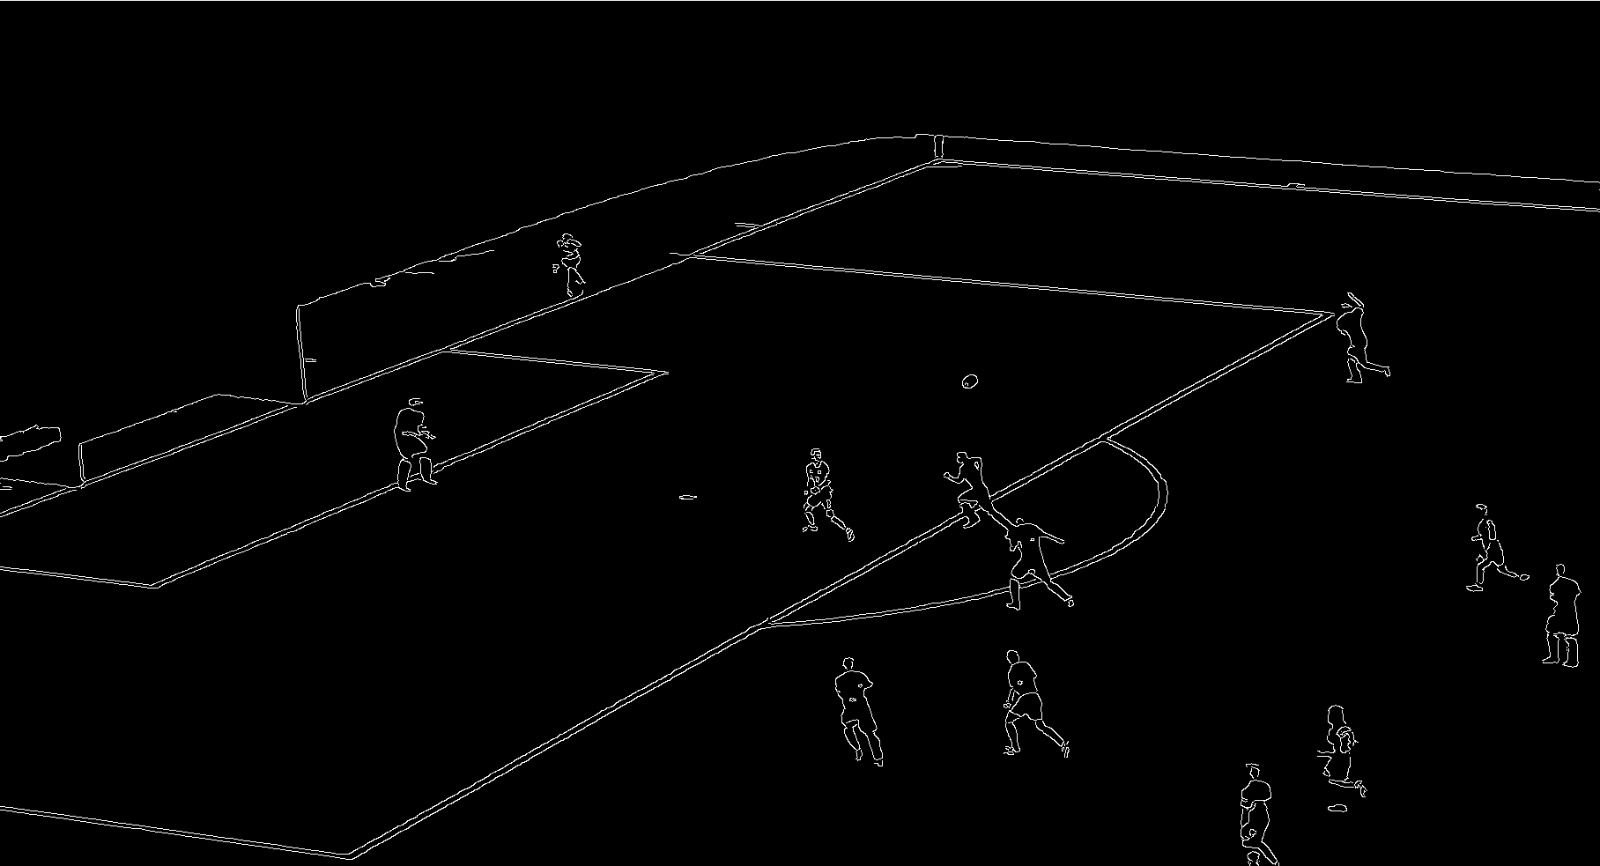
\includegraphics[width=\linewidth]{capitoli/cannyimage.jpeg}
        \subcaption{}
    \end{subfigure}
    \begin{subfigure}{0.40\textwidth}
        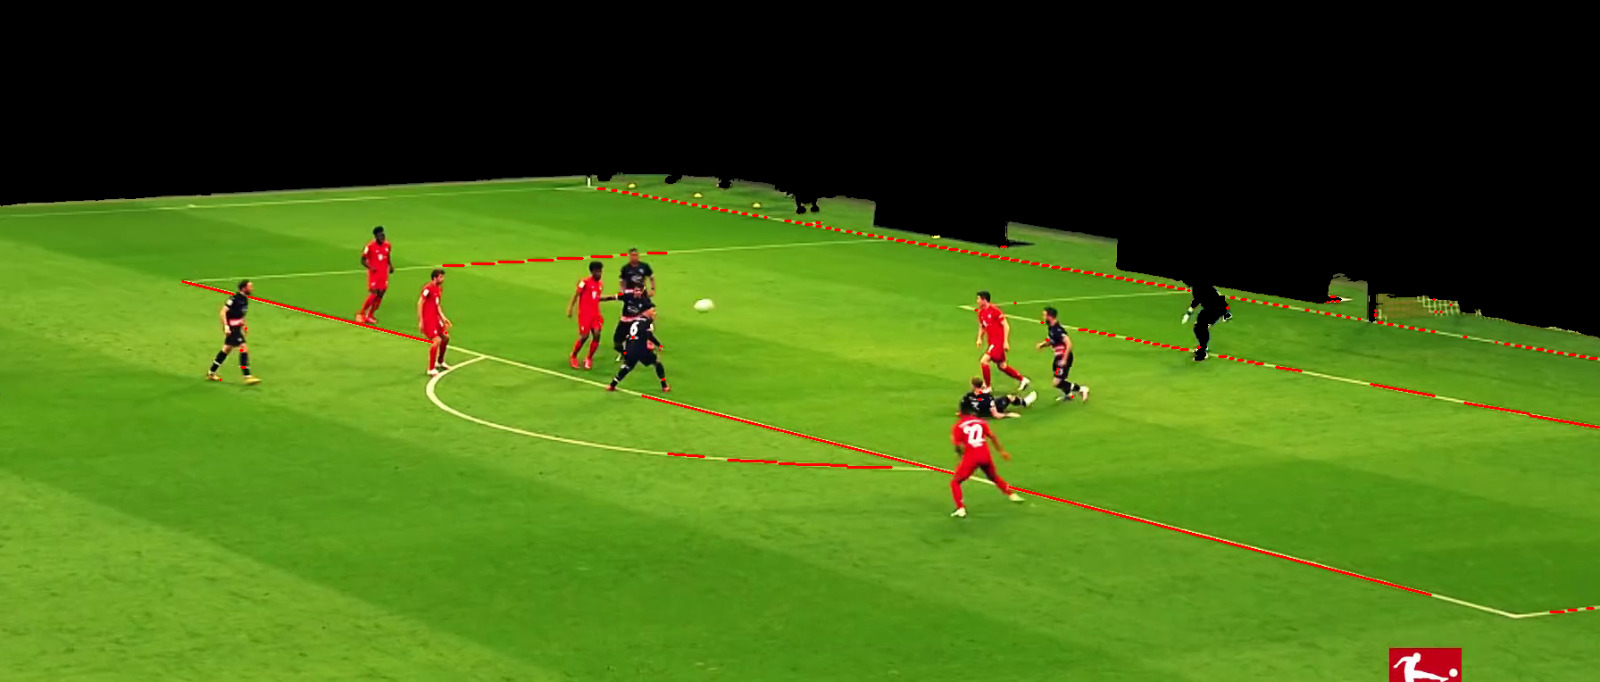
\includegraphics[width=\linewidth]{capitoli/roughlines.jpeg}
        \subcaption{}
    \end{subfigure}
    \caption{a: Immagine processata per facilitare l'individuamento delle linee maschere, b: Immagine risultante dopo aver applicato RoughLinesP}
    \label{fig:foobar}
\end{figure}

A seguito di questi problemi, è stato deciso di provare ad utilizzare un altro approccio, ovvero una soluzione che sfruttasse il \textbf{punto di fuoco} dell'immagine rispetto alla prospettiva, per alcuni punti fondamentali all'interno del campo, cosi da permetterci di effettuare una proiezione. 
In particolare, la soluzione da noi proposta cercava di tracciare delle linee nel campo in modo tale che fossero parallele o conformi alle linee del campo da calcio all'interno dell'immagine. Dopo aver individuato 2 linee principali, venivano prolungate fino a che non si fosse riscontrata un intersezione fra le due linee, ovvero il punto di fuoco.

\begin{figure}[h]
    \centering
    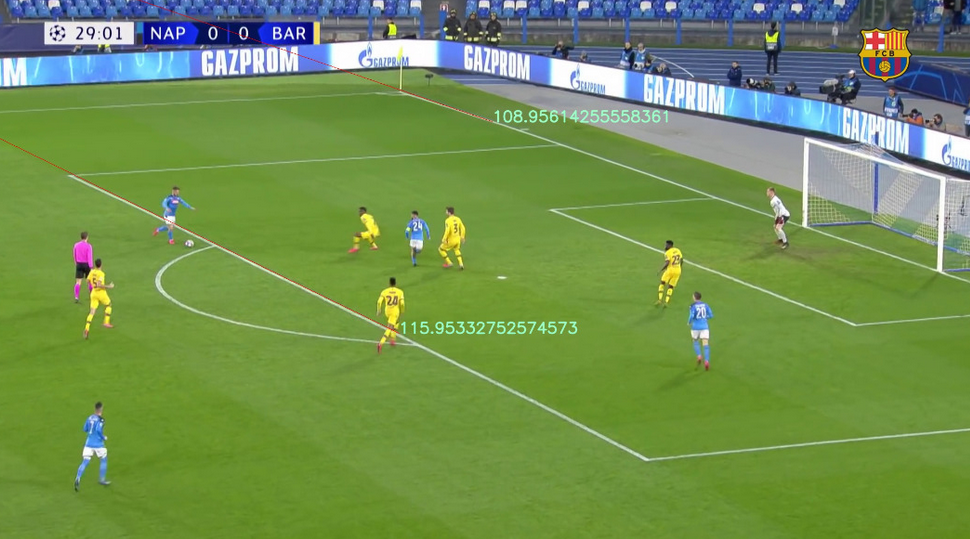
\includegraphics[width=0.7\linewidth]{capitoli/vanishingpoint.png}
    \caption{Immagine risultante dopo aver individuato il punto di fuoco, i numeri in verde sono i gradi della linea}
    \label{fig:enter-label}
\end{figure}

Anche questa metodologia riscontrava delle gravi problematiche, per immagini con prospettive molto orizzontali rispetto al campo, ovvero quando il punto di fuoco era presente all'interno dell'immagine, non era possibile individuare delle linee in modo corretto, ed inoltre non era possibile effettuare una proiezione 2D dei punti all'interno dell'immagine, essendo che le linee individuate erano in una posizione casuale dell'immagine. Quindi se avessimo dovuto solamente individuare il fuorigioco, la seguente metodologia avrebbe funzionato, però ai fini del nostro progetto era anche molto importante poter avere una rappresentazione 2D del campo e dei giocatori. Per questi motivi, è stato deciso di scartare anche questa opzione.
\\
\\

\subsection{Approccio finale}
Il metodo migliore che abbiamo trovato è stato l'utilizzo di un modello di Deep Learning [Bibliografia], che ci ha permesso di individuare la prospettiva corretta e di calcolare la matrice di omografia dell'immagine. Abbiamo dovuto adattare il modello per farlo lavorare su singoli frame, essendo stato creato per lavorare sui video.
\\ \\
Il modello in particolare ha come obiettivo l'utilizzo del Deep Learning [link wikipedia] per effettuare una regressione sugli errori, in modo da trovare i parametri di registrazione che minimizzano l'errore. Nello specifico propone una pipeline di reti neurali, che vengono utilizzate in modo sequenziale e ciclico. 
\\La prima rete neurale è chiamata \textit{Initial registration network}, permette di ottenere una stima dei parametri di registrazione e della corrispettiva matrice di omografia, fornendo in input alla rete neurale seguente, l'immagine presa in input e l'immagine di un campo 2D inserito in prospettiva tramite un warping nell'immagine in input, sfruttando i parametri e l'omografia ottenuti. 
\\La seconda rete neurale, viene chiamata \textit{Registration network error} e si occupa di minimizzare l'errore stimato dalla precedente rete, tramite una regressione. Nello specifico prende in ingresso i dati dalla rete neurale precedente, stima l'errore dell'omografia in base all'immagine presa come input, e tramite differenziazione e backpropagation, viene individuata la direzione nella quale l'errore viene minimizzato. La seguente operazione viene ripetuta iterativamente finché non viene raggiunto un obiettivo o non vengono raggiunte un numero prestabilito di operazioni.

\begin{figure}[h]
    \centering
    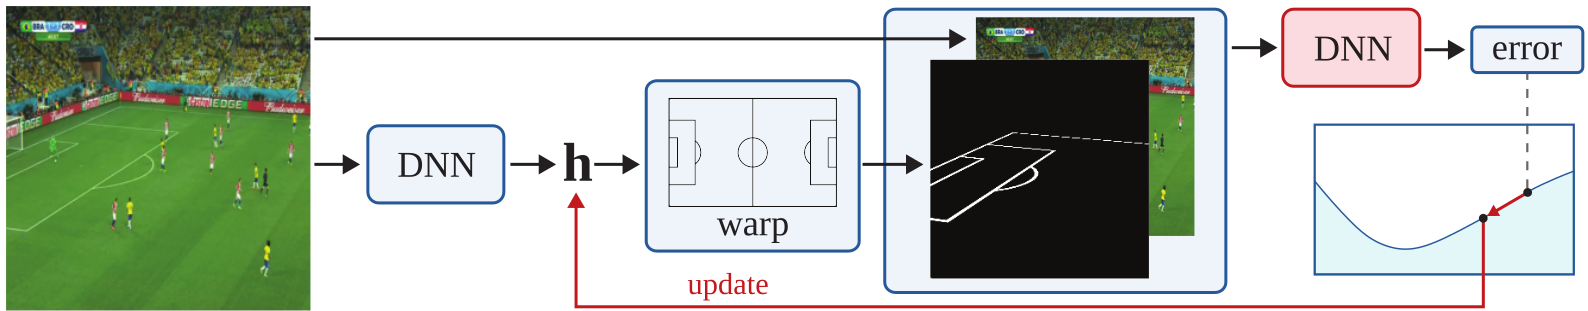
\includegraphics[width=1\linewidth]{capitoli/reteNeurale.png}
    \caption{Illustrazione del modello}
    \label{fig:enter-label}
\end{figure}

Possiamo quindi affermare in breve, che la prima rete neurale si occupa di fornire una stima approssimativa e non accurata della prospettiva e dell'omografia, ed in seguito, la seconda rete neurale si occupa di ottimizzare al massimo i parametri ottenuti, utilizzando un metodo che gli autori chiamano \textit{inference through optimization}, che permette di essere significativamente più accurati rispetto ai modelli classici che utilizzano il metodo del \textit{forwarding}.

Nello specifico, il metodo \textit{inference through optimization}, ha come scopo insegnare ad un modello a decretare quanto bene due immagini sono allineate. 
\\Il modello, a quanto affermato, è lo \textit{state-of-the-art} rispetto al dominio \textit{Camera calibration}, fornendo una stima molto accurata della prospettiva, gli autori affermano inoltre che il loro metodo di creazione del modello, è il primo che permette di imparare a regredire gli errori a partire da un immagine già ottimizzata.
\\\\
Un progetto affine al modello precedentemente descritto è il \textit{deep value network}, dove una rete neurale viene allenata per stimare la sezione di intersezione rispetto a due unioni, ovvero la stima del parametro \textit{IoU}.
\\È stato provato l'utilizzo di questo metodo, pero non ha fornito i risultati attesti e difatti, nel paper, gli autori esprimono il proprio giudizio riguardante il modello deep value network, in quanto esso, richiede una lunga ottimizzazione della traiettoria ed è inoltre limitato ad una sola iterazione iniziale, senza possibilità di miglioramenti.

\subsubsection{Dettagli pratici}

Per ottenere un omografia valida, è fondamentale avere un minimo di 4 punti non su una stessa linea. Il modello, come precedentemente descritto, crea una matrice di omografia fra l'immagine di gioco e il campo 2D, prendendo 4 punti che tipicamente contengono la visuale del campo dal basso, i punti sono descritti con i seguenti valori:
\begin{itemize}
    \item(-0.5, 0.1): angolo inferiore sinistro del rettangolo
    \item(-0.5, 0.5): angolo superiore sinistro del rettangolo
    \item(0.5, 0.5): angolo superiore destro del rettangolo
    \item(0.5, 0.1): angolo inferiore destro del rettangolo
\end{itemize}
\begin{figure}[h]
    \centering
    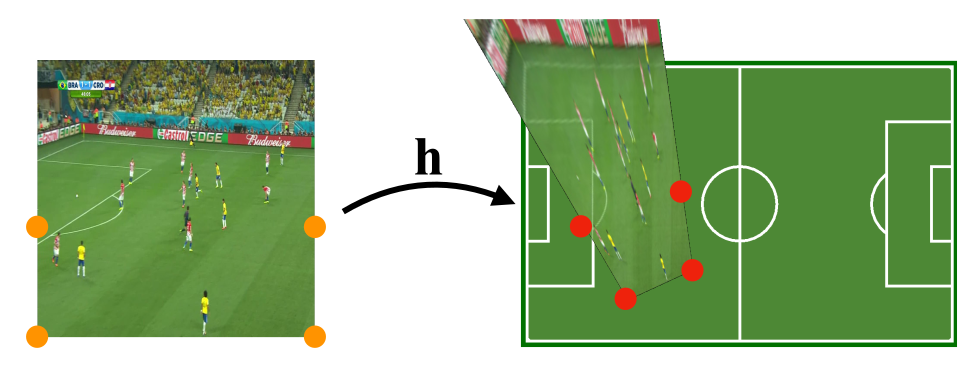
\includegraphics[width=0.7\linewidth]{capitoli/Hiniziale.png}
    \caption{Illustrazione dei punti di controllo per generare la matrice di omografia}
    \label{fig:enter-label}
\end{figure}
Andando a formare un lista \textbf{\begin{math}{h_{ref}}\end{math}} dove \begin{math}{u_1, v_1}\end{math} indicano la x e la y di un punto:
\[ \textbf{{\begin{math}{h_{ref}}\end{math}}} = [u_1, v_1, u_2, v_2, u_3, v_3, u_4, v_4 ] \]

Utilizzando i punti stimati in \textbf{{\begin{math}{h_{ref}}\end{math}}} e l'algoritmo di ottimizzazione \textbf{Adam}, è possibile ottenere una convergenza stabile durante l'ottimizzazione e quindi una matrice di omografia.
In particolare l'algoritmo Adam [Citazione al sito arxviv su algoritmo adam] permette di ottenere un ottimizzazione basata sul gradiente di primo ordine di una funzione. Questo algoritmo permette di addestrare modello di reti neurali, combinando i vantaggi di AdaGraf e RMSProp, adattando il learning rate per ciascun hyper-parameter. 
\\\\
I dataset utilizzati per validare ed addestrare il modello sono due.
Il primo è 'The World Cap dataset'[Link prendere dal paper], composto da 395 immagini divise fra training, validation e testing. Il secondo dataset è utilizzato riguarda la corrispondenza fra  il campo da calcio nell'immagine ed il template 2D, sono state utilizzate 39 immagini divise come per il precedente dataset fra training, validation e testing. 
I dati sono stati trattati con la tecnica del \textit{Data augmentation} per aumentare i sample e per migliorare il funzionamento del modello proponendo scenari e casistiche differenti.
\\\\
Entambi i modelli si basano su un architettura molto conosciuta, ovvero ResNet-18, opportunamente modificata dagli autori.
\begin{figure}[h]
    \centering
    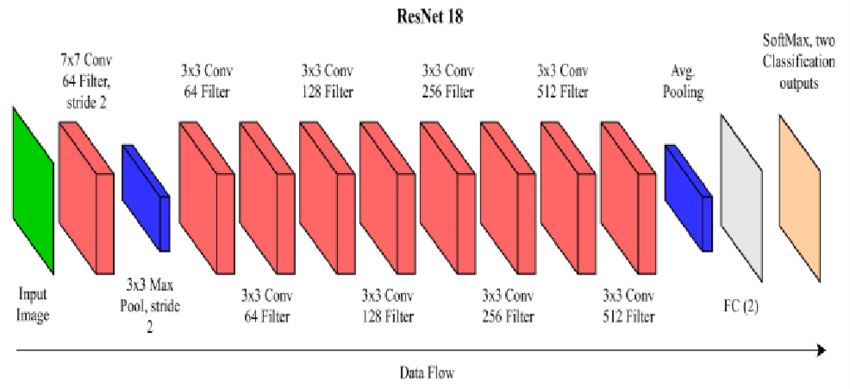
\includegraphics[width=0.7\linewidth]{capitoli/resnetArch.png}
    \caption{Illustrazione dell'architettura}
    \label{fig:enter-label}
\end{figure}

Nel primo modello, è stata sostituita la parte finale, ovvero la testa, con un ultimo layer nella quale convergono tutti i nodi della rete (fully connected layer), utilizzato per stimare gli 8 numeri che vanno poi a rappresentare l'omografia.
Nel secondo modello su tutti i livelli è stata applicata una spectral normalization, ovvero una tecnica di normalizzazione utilizzata per stabilizzare l'allenamento del discriminante [link paperwithcode].
Sull'ultimo livello (head) è stata applicata una funzione \textit{sigmoid} per rendere il risultato positivo, ed una funzione per la riproiezione dell'errore metrico.

\subsubsection{Risultati}

I risultati del modello sono eccellenti, come si può evincere dal risultato [Fig 7], l'ottimizzazione è un fattore chiave per la precisione finale, dovendo effettuare un training personalizzato su ogni immagine che viene inserita in input, rendendo cosi la velocità del modello dipendente dall'hardware della macchina. 


\begin{figure}[h]
    \centering
    \begin{subfigure}{0.45\textwidth}
        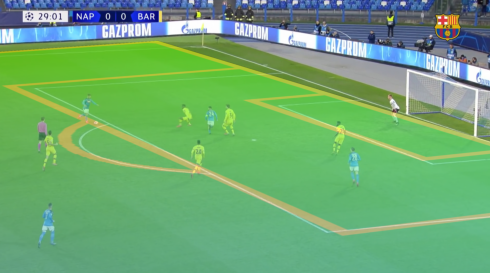
\includegraphics[width=\linewidth]{capitoli/HpitchSample.png}
        \subcaption{}
    \end{subfigure}
    \begin{subfigure}{0.45\textwidth}
        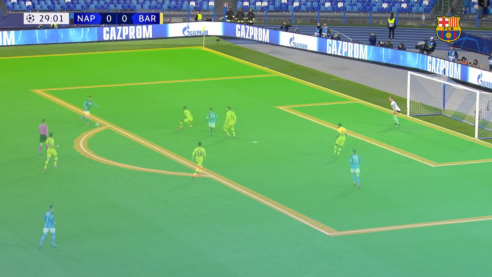
\includegraphics[width=\linewidth]{capitoli/HpitchOptimSample.png}
        \subcaption{}
    \end{subfigure}
    \caption{a: Immagine iniziale derivante dal primo modello, b: Immagine risultante dopo l'ottimizzazione tramite 200 iterazioni}
    \label{fig:foobar}
\end{figure}

 Un miglioramento che si potrebbe attuare al modello sarebbe la sostituzione della seconda parte, l'ottimizzazione, che rende tutto il processo di lavorazione dell'immagine molto lento, a favore di un miglioramento del primo modello, tramite per esempio un cambio architettura alla base. 
\\\\
 In conclusione, il modello ci ha permesso di ottenere i dati che servivano al progetto, ovvero la matrice di omografia, per effettuare una corrispondenza quanto più precisa possibile dei punti in 3D su un template 2D.

\end{document}

\section{GUI}
\input{capitoli/gui.tex}
\input{capitoli/offside.tex}

\section{Citations and Bibliographies}

The use of \BibTeX\ for the preparation and formatting of one's
references is strongly recommended. Authors' names should be complete
--- use full first names (``Donald E. Knuth'') not initials
(``D. E. Knuth'') --- and the salient identifying features of a
reference should be included: title, year, volume, number, pages,
article DOI, etc.

The bibliography is included in your source document with these two
commands, placed just before the \verb|\end{document}| command:
\begin{verbatim}
  \bibliographystyle{ACM-Reference-Format}
  \bibliography{bibfile}
\end{verbatim}
where ``\verb|bibfile|'' is the name, without the ``\verb|.bib|''
suffix, of the \BibTeX\ file.

Citations and references are numbered by default. A small number of
ACM publications have citations and references formatted in the
``author year'' style; for these exceptions, please include this
command in the {\bfseries preamble} (before the command
``\verb|\begin{document}|'') of your \LaTeX\ source:
\begin{verbatim}
  \citestyle{acmauthoryear}
\end{verbatim}


  Some examples.  A paginated journal article \cite{Abril07}, an
  enumerated journal article \cite{Cohen07}, a reference to an entire
  issue \cite{JCohen96}, a monograph (whole book) \cite{Kosiur01}, a
  monograph/whole book in a series (see 2a in spec. document)
  \cite{Harel79}, a divisible-book such as an anthology or compilation
  \cite{Editor00} followed by the same example, however we only output
  the series if the volume number is given \cite{Editor00a} (so
  Editor00a's series should NOT be present since it has no vol. no.),
  a chapter in a divisible book \cite{Spector90}, a chapter in a
  divisible book in a series \cite{Douglass98}, a multi-volume work as
  book \cite{Knuth97}, a couple of articles in a proceedings (of a
  conference, symposium, workshop for example) (paginated proceedings
  article) \cite{Andler79, Hagerup1993}, a proceedings article with
  all possible elements \cite{Smith10}, an example of an enumerated
  proceedings article \cite{VanGundy07}, an informally published work
  \cite{Harel78}, a couple of preprints \cite{Bornmann2019,
    AnzarootPBM14}, a doctoral dissertation \cite{Clarkson85}, a
  master's thesis: \cite{anisi03}, an online document / world wide web
  resource \cite{Thornburg01, Ablamowicz07, Poker06}, a video game
  (Case 1) \cite{Obama08} and (Case 2) \cite{Novak03} and \cite{Lee05}
  and (Case 3) a patent \cite{JoeScientist001}, work accepted for
  publication \cite{rous08}, 'YYYYb'-test for prolific author
  \cite{SaeediMEJ10} and \cite{SaeediJETC10}. Other cites might
  contain 'duplicate' DOI and URLs (some SIAM articles)
  \cite{Kirschmer:2010:AEI:1958016.1958018}. Boris / Barbara Beeton:
  multi-volume works as books \cite{MR781536} and \cite{MR781537}. A
  couple of citations with DOIs:
  \cite{2004:ITE:1009386.1010128,Kirschmer:2010:AEI:1958016.1958018}. Online
  citations: \cite{TUGInstmem, Thornburg01, CTANacmart}.
  Artifacts: \cite{R} and \cite{UMassCitations}.

\section{Acknowledgments}

Identification of funding sources and other support, and thanks to
individuals and groups that assisted in the research and the
preparation of the work should be included in an acknowledgment
section, which is placed just before the reference section in your
document.

This section has a special environment:
\begin{verbatim}
  \begin{acks}
  ...
  \end{acks}
\end{verbatim}
so that the information contained therein can be more easily collected
during the article metadata extraction phase, and to ensure
consistency in the spelling of the section heading.

Authors should not prepare this section as a numbered or unnumbered {\verb|\section|}; please use the ``{\verb|acks|}'' environment.

\section{Appendices}

If your work needs an appendix, add it before the
``\verb|\end{document}|'' command at the conclusion of your source
document.

Start the appendix with the ``\verb|appendix|'' command:
\begin{verbatim}
  \appendix
\end{verbatim}
and note that in the appendix, sections are lettered, not
numbered. This document has two appendices, demonstrating the section
and subsection identification method.

\section{Multi-language papers}

Papers may be written in languages other than English or include
titles, subtitles, keywords and abstracts in different languages (as a
rule, a paper in a language other than English should include an
English title and an English abstract).  Use \verb|language=...| for
every language used in the paper.  The last language indicated is the
main language of the paper.  For example, a French paper with
additional titles and abstracts in English and German may start with
the following command
\begin{verbatim}
\documentclass[sigconf, language=english, language=german,
               language=french]{acmart}
\end{verbatim}

The title, subtitle, keywords and abstract will be typeset in the main
language of the paper.  The commands \verb|\translatedXXX|, \verb|XXX|
begin title, subtitle and keywords, can be used to set these elements
in the other languages.  The environment \verb|translatedabstract| is
used to set the translation of the abstract.  These commands and
environment have a mandatory first argument: the language of the
second argument.  See \verb|sample-sigconf-i13n.tex| file for examples
of their usage.

\section{SIGCHI Extended Abstracts}

The ``\verb|sigchi-a|'' template style (available only in \LaTeX\ and
not in Word) produces a landscape-orientation formatted article, with
a wide left margin. Three environments are available for use with the
``\verb|sigchi-a|'' template style, and produce formatted output in
the margin:
\begin{description}
\item[\texttt{sidebar}:]  Place formatted text in the margin.
\item[\texttt{marginfigure}:] Place a figure in the margin.
\item[\texttt{margintable}:] Place a table in the margin.
\end{description}

%%
%% The acknowledgments section is defined using the "acks" environment
%% (and NOT an unnumbered section). This ensures the proper
%% identification of the section in the article metadata, and the
%% consistent spelling of the heading.
\begin{acks}
To Robert, for the bagels and explaining CMYK and color spaces.
\end{acks}

%%
%% The next two lines define the bibliography style to be used, and
%% the bibliography file.
\bibliographystyle{ACM-Reference-Format}
\bibliography{sample-base}


%%
%% If your work has an appendix, this is the place to put it.
\appendix

\section{Research Methods}

\subsection{Part One}

Lorem ipsum dolor sit amet, consectetur adipiscing elit. Morbi
malesuada, quam in pulvinar varius, metus nunc fermentum urna, id
sollicitudin purus odio sit amet enim. Aliquam ullamcorper eu ipsum
vel mollis. Curabitur quis dictum nisl. Phasellus vel semper risus, et
lacinia dolor. Integer ultricies commodo sem nec semper.

\subsection{Part Two}

Etiam commodo feugiat nisl pulvinar pellentesque. Etiam auctor sodales
ligula, non varius nibh pulvinar semper. Suspendisse nec lectus non
ipsum convallis congue hendrerit vitae sapien. Donec at laoreet
eros. Vivamus non purus placerat, scelerisque diam eu, cursus
ante. Etiam aliquam tortor auctor efficitur mattis.

\section{Online Resources}

Nam id fermentum dui. Suspendisse sagittis tortor a nulla mollis, in
pulvinar ex pretium. Sed interdum orci quis metus euismod, et sagittis
enim maximus. Vestibulum gravida massa ut felis suscipit
congue. Quisque mattis elit a risus ultrices commodo venenatis eget
dui. Etiam sagittis eleifend elementum.

Nam interdum magna at lectus dignissim, ac dignissim lorem
rhoncus. Maecenas eu arcu ac neque placerat aliquam. Nunc pulvinar
massa et mattis lacinia.

\end{document}
\endinput
%%
%% End of file `sample-acmtog.tex'.
